\chapter{Fazit}
Der HMF-Gehalt aller vermessenen unbehandelten Honige waren bezüglich der staatlichen Vorgaben unbedenklich. Selbst der Honig 4, der das Mindesthaltbarkeitsdatum bereits überschritten hatte, blieb innerhalb der Grenzwerte. Allerdings war ein Großteil bereits auskristallisiert. Somit war die vermessene Probe inhomogen. Es kann nicht ausgeschlossen werden, dass ein erhöhter HMF-Gehalt in den kristallisierten Rückständen vorliegt.\\
\begin{figure}[htbp]
  \centering
  \subfigure[Vorderseite]{
    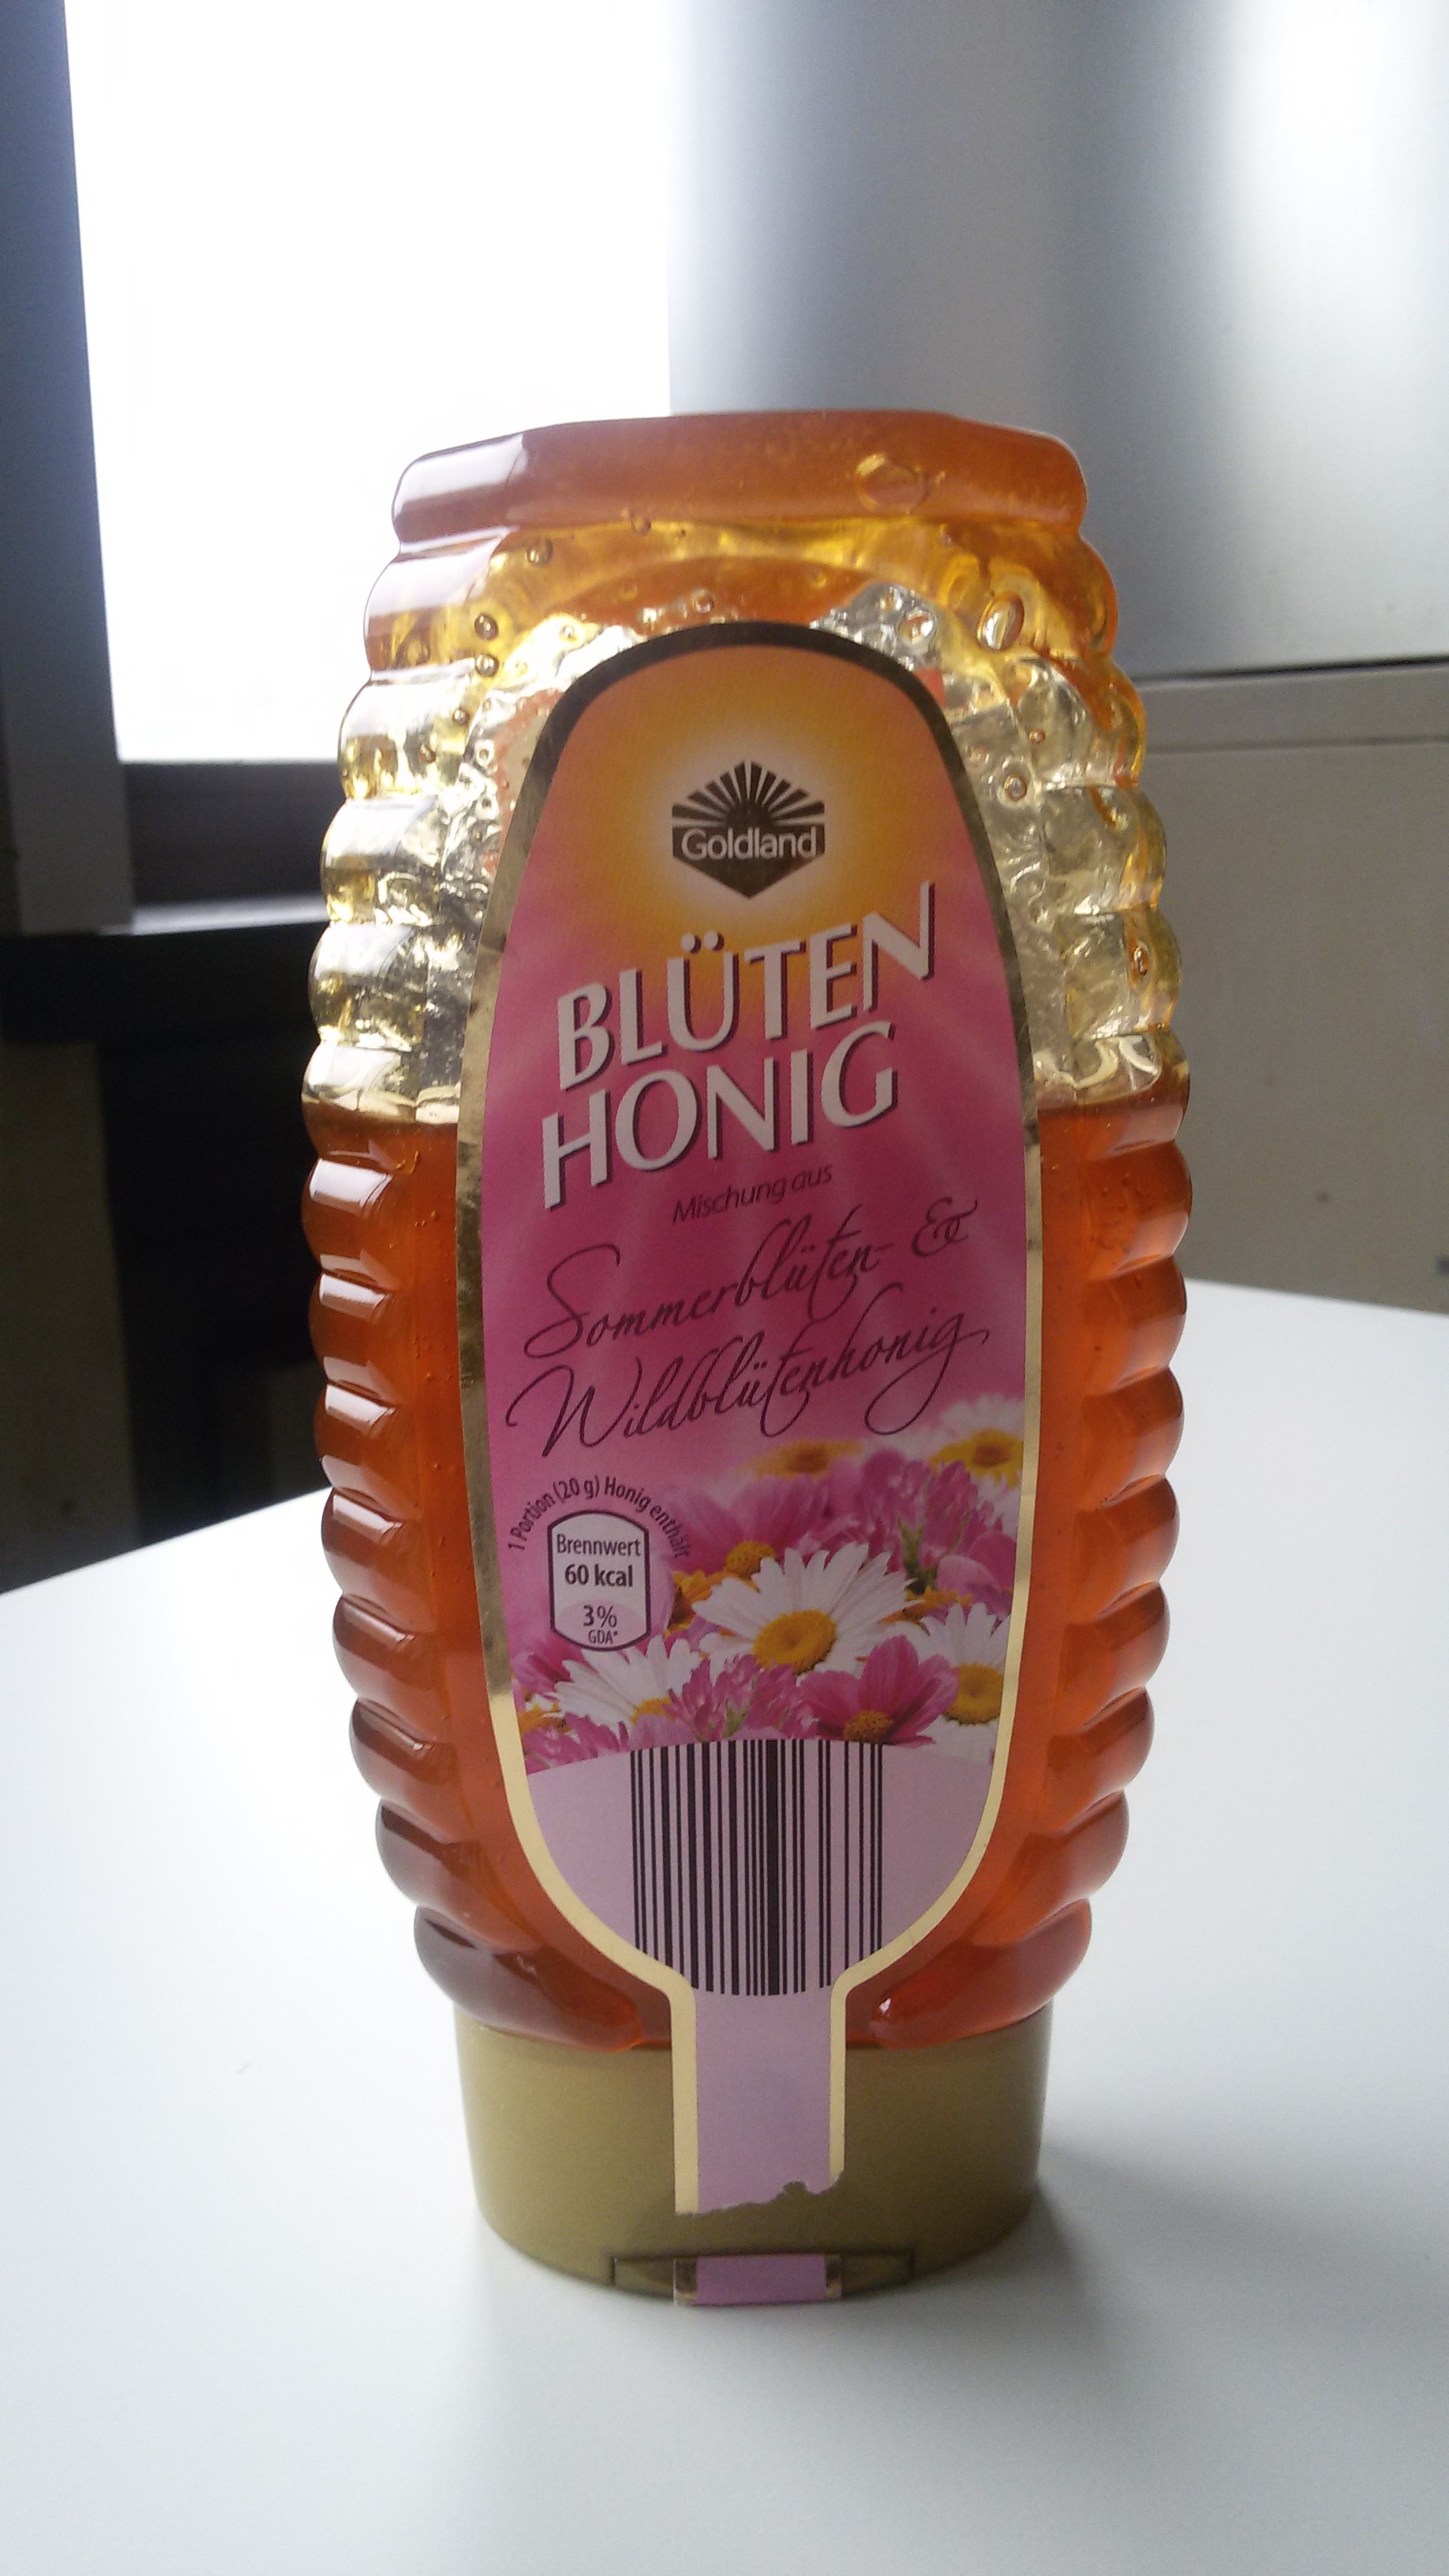
\includegraphics[]{../Bilder/20150416_182012.jpg}
  }
  \subfigure[Rückseite]{
    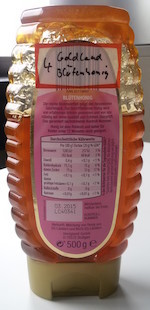
\includegraphics{../Bilder/20150416_182004.jpg}
  }
  \caption{Blütenhonig Goldland}
  \label{fig:Blütenhonig}
\end{figure}

Der Invertzucker überraschte mit seinem hohen HMF-Gehalt von ca. 300mg/kg. Dies erklärt sich durch sein Herstellungsverfahren bei dem eine Saccharoselösung mit Zitronensäure gekocht wird.\\
Erstaunlicherweise war der mexikanische Honig nicht auffällig. Da für Tropenhonige deutlich höhere zulässige Grenzwerte gelten, erwarteten wir auch einen deutlich erhöhten HMF-Gehalt. \\
Der Sommerblütenhonig der Firma ''Vom Land'' (Probe 3 \ref{tab:Messergebnisse}) zeigt den höchsten HMF-Gehalt mit ca. 30mg/kg. Die Probe war nahe dem Verfallsdatum, hatte dieses aber noch nicht überschritten.\\
Der thermische Einfluss auf die Honige führte zu einem deutlichen Anstieg des HMF-Gehalts. Die Konzentrationen bewegten sich bei allen Honigen bei ca. 250mg/kg. Da alle Honige für die gleiche Zeitspanne temperiert wurden, kann man annehmen, dass die Entstehungsrate von HMF bei allen Proben annähernd identisch ist. Eine Ausnahme bildet der Sommerblütenhonig, bei dem der HMF-Gehalt mit 379mg/kg außerhalb des linearen Messbereichs liegt. Somit kann keine exakte Aussage über die HMF Bildung in der Probe 3 getroffen werden. Allerdings korreliert dieser hohe Wert mit dem gefunden HMF-Gehalt in der unbehandelten Probe 3.\\
Das Winterfutter wies einen äußerst niedrigen HMF-Gehalt auf. Dies zeigt, dass der Imker in der Winterphase den Bienenstock nicht zusätzlich erwärmt hat. Das Wärmen erniedrigt den Energieaufwand, den die Bienen im Winter erbringen müssen um ihren Stock warm zu halten. Höhere Temperaturen im Stock führen zu einem frühen Brüten der Bienen.\\
Vergleicht man die über die Kalibrierung ermittelten Werte mit den über den Festfaktor berechneten, so zeigt sich das die berechneten Werte höher sind. Die Ursache hierfür ist wahrscheinlich ein systematischer Fehler, da die Kalibriergerade mit einem Bestimmtheitsmaß von 0,9997 in sich schlüssig ist. Der Grund dafür könnte sein, dass nicht alle Matrixbestandteile bei der Fällung und anschließender Filtration abgetrennt werden konnten.\\
Eine verwendbare Kalibriergerade konnte erst im zweiten Versuch erstellt werden. Beim ersten Vermessen der Kalibrierlösungen wurde nicht die enorme Zerfallsrate des Farbkomplexes berücksichtigt. Nach WINKLER besteht nur ein Zeitfenster von einer Minute um die Messung durchzuführen.~\cite{Winkler} Die nicht verwendete Kalibriergerade ist im Anhang hinzugefügt.\\
Im allgemeinen lässt sich erkennen, dass die verwendete Methode sehr genaue Messergebnisse liefert. Dies hat die Bestimmung der Wiederfindung, sowie die Ermittelung der Standardabweichung nach mehrfacher Bestimmung gezeigt.\\
Der Rübensirup der Firma ''Grafschafter'' (Probe 8) war nicht zur Vermessung geeignet. Zum einen war die Eigenfärbung dunkelbraun bis tiefschwarz. Eine Lichtdurchlässigkeit war unwahrscheinlich. Bei der Filtration setzten sich die Poren des Filters sofort zu. Es konnte kein Filtrat gewonnen werden.\\
\begin{figure}[htbp]
  \centering
  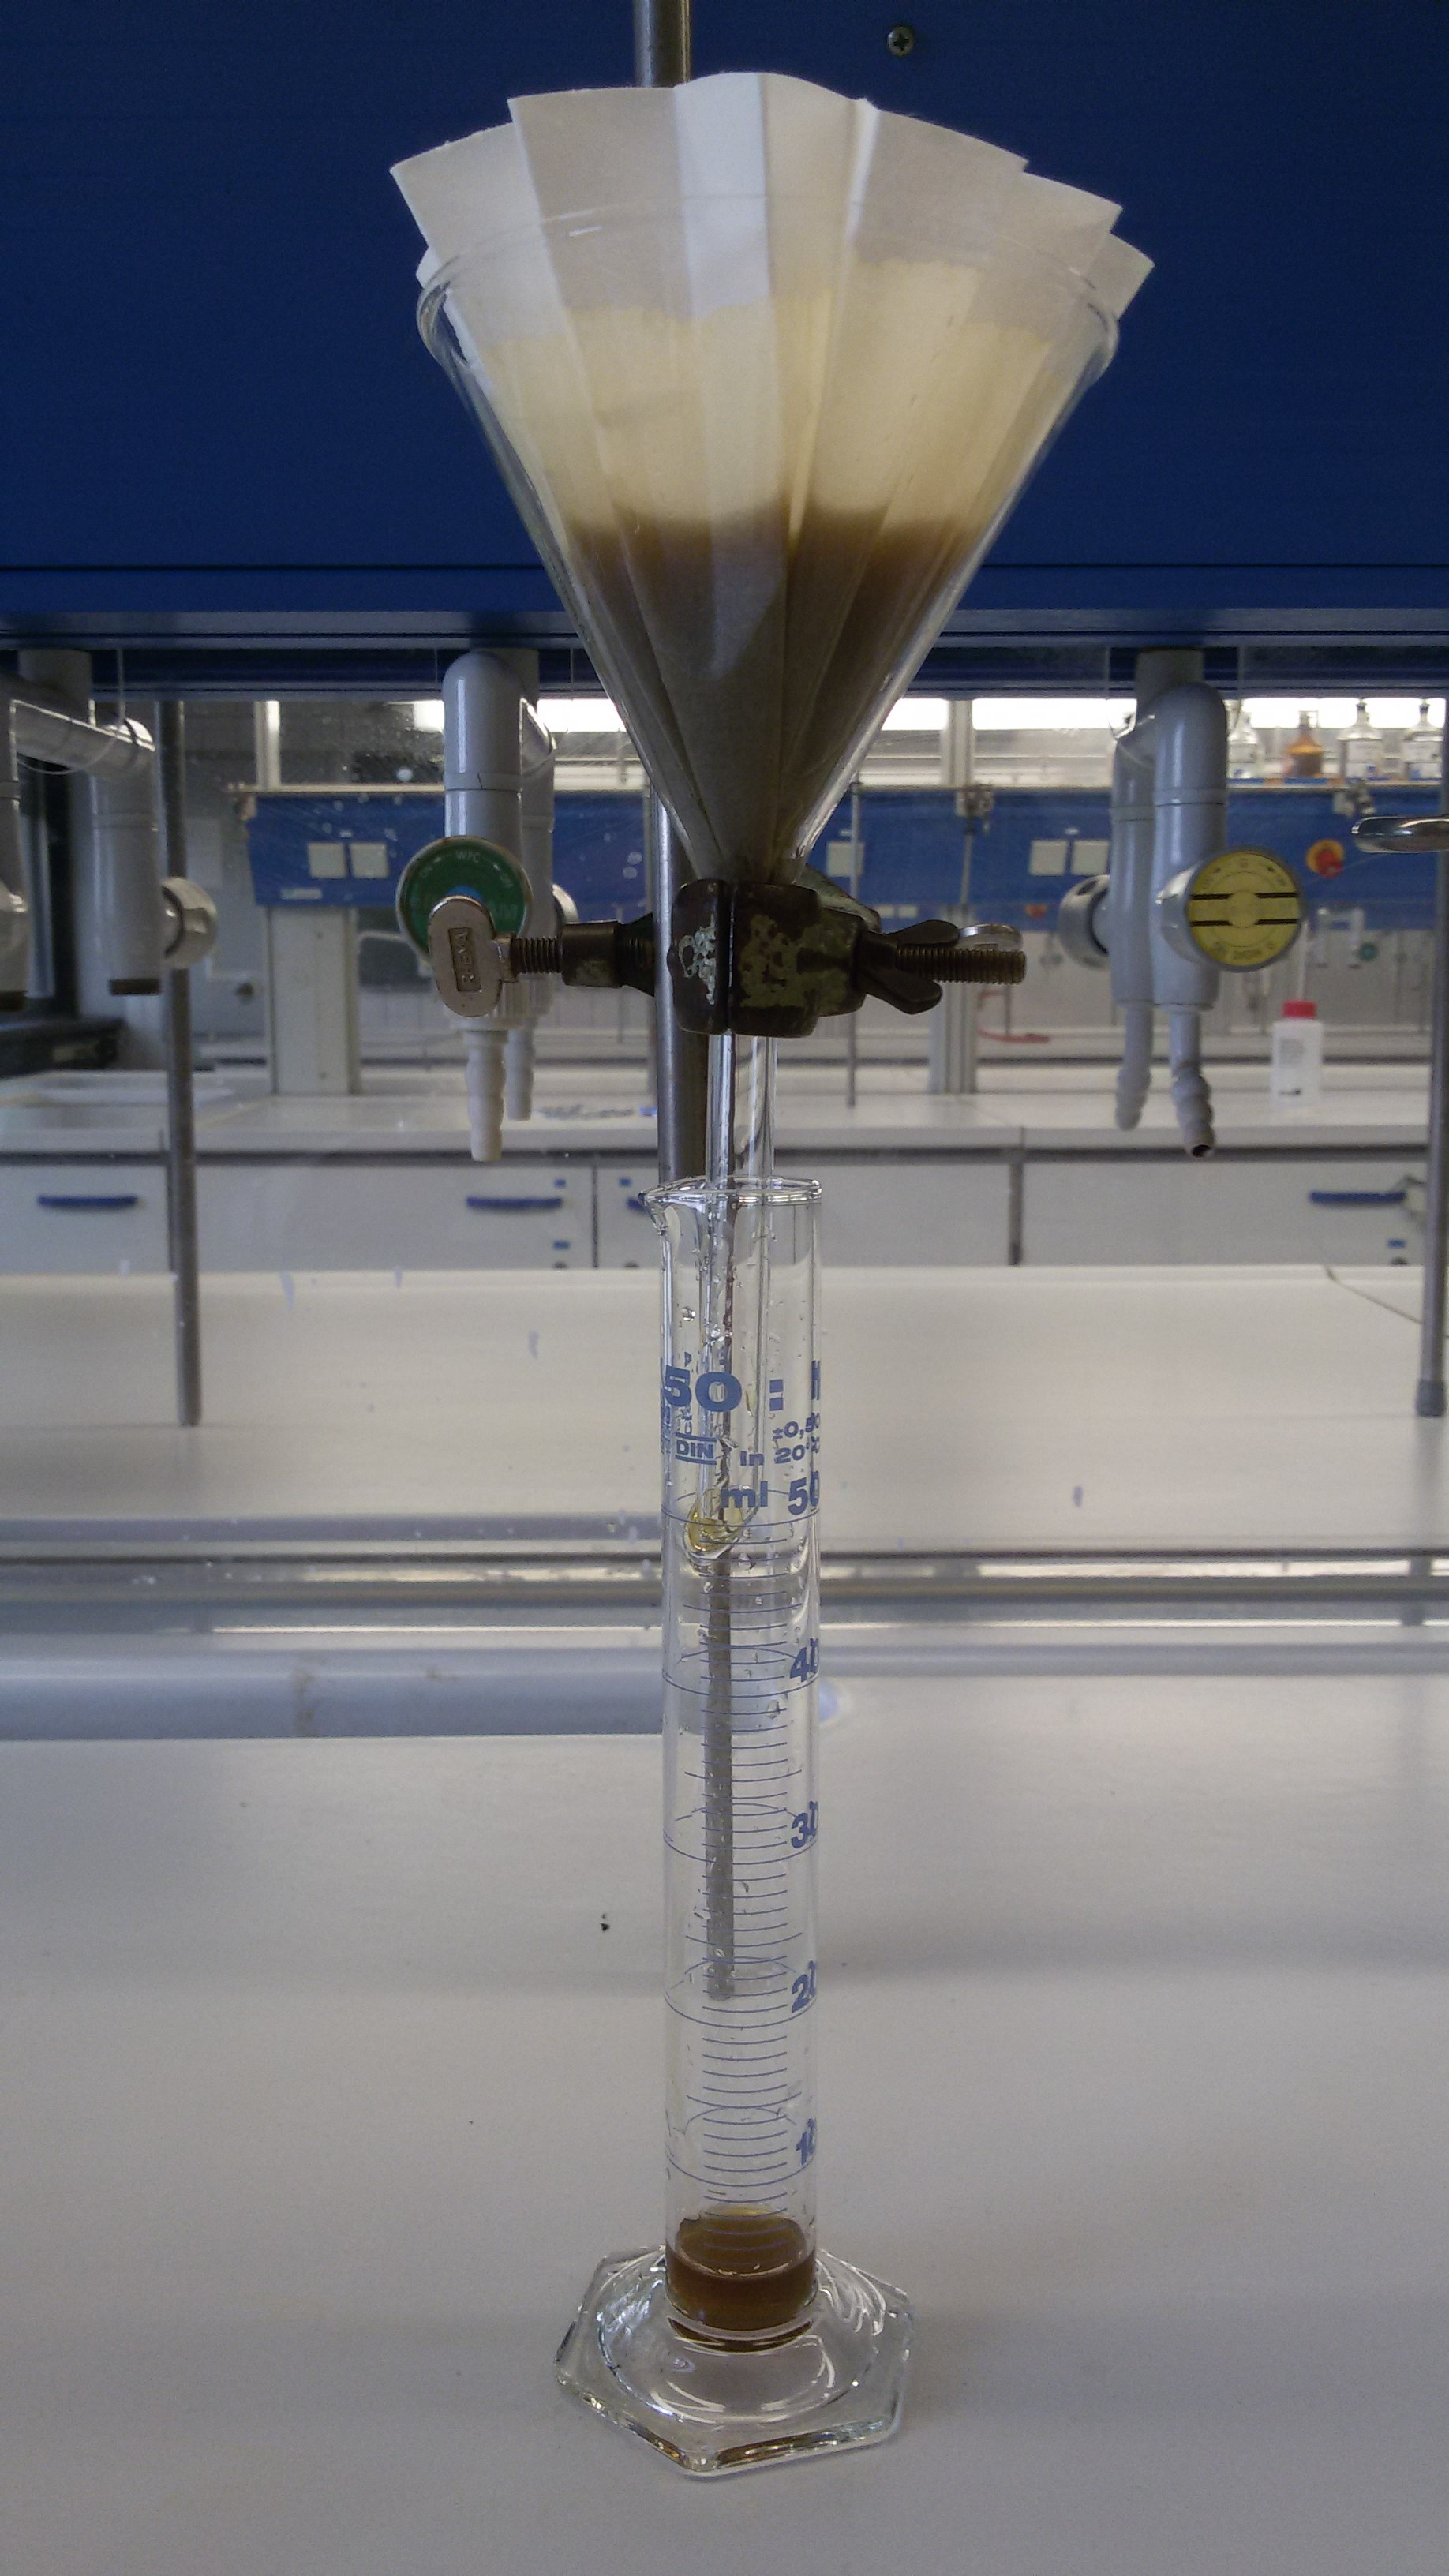
\includegraphics[width=1.00\textwidth]{../Bilder/20150427_153416.jpg}
  \caption{Filtrationsversuch Grafschafter}
  \label{fig:Grafschafter}
\end{figure}
Die durchgeführten Versuche zeigen einen ersten Einblick in das Zusammenwirken von Fruchtzucker und HMF bei thermischer Belastung, sowie bei Raumtemperatur. Zahlreiche Einflussfaktoren blieben bei den Versuchen jedoch bislang unberücksichtigt. So liegen keine Erkenntnisse über den Zusammenhang von pH-Wert, Wassergehalt und Enzymtätigkeit mit der Bildung von HMF vor. Außerdem ist nicht bekannt, ob der gesamte Fruchtzucker in Honig zu HMF umgewandelt werden kann, oder ob sich bei hoher Konzentration ein Gleichgewicht einstellt. Hierfür müssten weitere Untersuchungen, auch über einen längeren Zeitraum, durchgeführt werden.
